%
% The first command in your LaTeX source must be the \documentclass command.
\documentclass[sigconf]{acmart}

\hypersetup{draft}
% For links
\PassOptionsToPackage{hyphens}{url}
%\PassOptionsToPackage{draft}{hyperref}
\usepackage{hyperref}
\usepackage{url}
% originally to compile w/ correct hyperlinks, needed: 
% latex -> bibtex -> latex -> latex -> dvi2ps -> ps2pdf
% now PDFLaTeX seems to work.
\usepackage{subcaption}

% defining the \BibTeX command - from Oren Patashnik's original BibTeX documentation.
\def\BibTeX{{\rm B\kern-.05em{\sc i\kern-.025em b}\kern-.08emT\kern-.1667em\lower.7ex\hbox{E}\kern-.125emX}}
    
% Rights management information. 
% This information is sent to you when you complete the rights form.
% These commands have SAMPLE values in them; it is your responsibility as an author to replace
% the commands and values with those provided to you when you complete the rights form.

% These commands are for a PROCEEDINGS abstract or paper.
\copyrightyear{\url{https://fatconference.org/2020/callfortutorials.html}}
\acmYear{}
\setcopyright{none}
\acmConference[ACM FAT* Call for Tutorials -- \textit{UNDER REVIEW}]{ACM FAT* Conference 2020}{Barcelona}{2020}
\acmBooktitle{ACM FAT* Conference, Jan. 27\textsuperscript{th} -- 30\textsuperscript{th}, 2020, Barcelona, Spain}
\acmPrice{}
\acmDOI{}
\acmISBN{}

% These commands are for a JOURNAL article.
%\setcopyright{acmcopyright}
%\acmJournal{TOG}
%\acmYear{2018}\acmVolume{37}\acmNumber{4}\acmArticle{111}\acmMonth{8}
%\acmDOI{10.1145/1122445.1122456}


% Submission ID. 
% Use this when submitting an article to a sponsored event. You'll receive a unique submission ID from the organizers
% of the event, and this ID should be used as the parameter to this command.
%\acmSubmissionID{123-A56-BU3}


% The majority of ACM publications use numbered citations and references. If you are preparing content for an event
% sponsored by ACM SIGGRAPH, you must use the "author year" style of citations and references. Uncommenting
% the next command will enable that style.
%\citestyle{acmauthoryear}

%two part definition
\newcommand{\twopartdef}[4]
{
	\left\{
		\begin{array}{ll}
			#1 & \mbox{if } #2 \\
			#3 & \mbox{if } #4
		\end{array}
	\right.
}

% end of the preamble, start of the body of the document source.
\begin{document}

% The "title" command has an optional parameter, allowing the author to define a "short title" to be used in page headers.
\title[Responsible XAI]{\huge{Hands-On Tutorial: Responsible Use Guidelines for\\ Explainable Machine Learning}}


% The "author" command and its associated commands are used to define the authors and their affiliations.
% Of note is the shared affiliation of the first two authors, and the "authornote" and "authornotemark" commands
% used to denote shared contribution to the research.
\author{Patrick Hall}
\email{patrick.hall@h2o.ai}
\affiliation{\institution{H2O.ai}}
\affiliation{\institution{George Washington University}}

\author{Navdeep Gill}
\email{navdeep.gill@h2o.ai}
\affiliation{\institution{H2O.ai}}

\author{Nicholas Schmidt }
\email{nschmidt@bldsllc.com}
\affiliation{\institution{BLDS, LLC}}

\renewcommand{\shortauthors}{Hall, Gill, \& Schmidt}

%
% The abstract is a short summary of the work to be presented in the article.
%\begin{abstract}
%\end{abstract}

%
% The code below is generated by the tool at http://dl.acm.org/ccs.cfm.
% Please copy and paste the code instead of the example below.
%
%\begin{CCSXML}
%	<ccs2012>

%		<concept>
%			<concept_id>10003120.10003145.10003147.10010365</concept_id>
%			<concept_desc>Human-centered computing~Visual analytics</concept_desc>
%			<concept_significance>300</concept_significance>
%		</concept>		

%		<concept>
%			<concept_id>10010147.10010257.10010258.10010259.10010263</concept_id>
%			<concept_desc>Computing methodologies~Supervised learning by classification</concept_desc>
%			<concept_significance>300</concept_significance>
%		</concept>

%		<concept>
%			<concept_id>10010147.10010257.10010258.10010259.10010264</concept_id>
%			<concept_desc>Computing methodologies~Supervised learning by regression</concept_desc>
%			<concept_significance>300</concept_significance>
%		</concept>
		
%		<concept>
%			<concept_id>10010147.10010257.10010293.10010307</concept_id>
%			<concept_desc>Computing methodologies~Learning linear models</concept_desc>
%			<concept_significance>300</concept_significance>
%		</concept>
		
%		<concept>
%			<concept_id>10010147.10010257.10010293.10003660</concept_id>
%			<concept_desc>Computing methodologies~Classification and regression trees</concept_desc>
%			<concept_significance>300</concept_significance>
%		</concept>

%		<concept>
%			<concept_id>10010147.10010257.10010321.10010333</concept_id>
%			<concept_desc>Computing methodologies~Ensemble methods</concept_desc>
%			<concept_significance>300</concept_significance>
%		</concept>		
				
%	</ccs2012>
%\end{CCSXML}

%\ccsdesc[300]{Human-centered computing~Visual analytics}
%\ccsdesc[300]{Computing methodologies~Supervised learning by classification}
%\ccsdesc[300]{Computing methodologies~Supervised learning by regression}
%\ccsdesc[300]{Computing methodologies~Learning linear models}
%\ccsdesc[300]{Computing methodologies~Classification and regression trees}
%\ccsdesc[300]{Computing methodologies~Ensemble methods}

%
% Keywords. The author(s) should pick words that accurately describe the work being
% presented. Separate the keywords with commas.
%\keywords{Machine learning, interpretability, explanations, transparency,\\ FATML, XAI}


% This command processes the author and affiliation and title information and builds
% the first part of the formatted document.
\maketitle

%-------------------------------------------------------------------------------
\section*{Introduction \& Agenda}
%-------------------------------------------------------------------------------

Explainable machine learning (ML) enables human learning from ML, human appeal of incorrect ML decisions, regulatory compliance, and security audits of ML models.\footnote{In the U.S., interpretable models, explainable ML, and model documentation they enable may be required under the Civil Rights Acts of 1964 and 1991, the Americans with Disabilities Act, the Genetic Information Nondiscrimination Act, the Health Insurance Portability and Accountability Act, the Equal Credit Opportunity Act (ECOA), the Fair Credit Reporting Act (FCRA), the Fair Housing Act, Federal Reserve SR 11-7, and the European Union (EU) Greater Data Privacy Regulation (GDPR) Article 22 \cite{ff_interpretability}. \label{fn:regs}} \textsuperscript{,}\footnote{For security applications, see for instance: \url{https://www.oreilly.com/ideas/proposals-for-model-vulnerability-and-security}.\label{fn:regs}} Explainable ML (i.e. e\textit{x}plainable \textit{a}rtificial \textit{i}ntelligence or XAI) has been implemented in numerous open source and commercial packages and explainable ML is also an important, mandatory, or embedded aspect of commercial predictive modeling in industries like financial services.\footnote{Like H2O-3, XGBoost, and various other Python and R packages. See: \url{https://github.com/jphall663/awesome-machine-learning-interpretability} for a longer, curated list of relevant open source software packages.}\textsuperscript{,}\footnote{For instance  Datarobot, H2O Driverless AI, SAS Visual Data Mining and Machine Learning, Zest AutoML, and likely several others.}\textsuperscript{,}\footnote{For instance, ``Deep Insights into Explainability and Interpretability of Machine Learning Algorithms and Applications to Risk Management,'' Jie Chen, Wells Fargo Corporate Model Risk, \url{https://ww2.amstat.org/meetings/jsm/2019/onlineprogram/AbstractDetails.cfm?abstractid=303053}. \label{fn:Chen}} However, like many technologies, explainable ML can be misused and abused, particularly as a faulty safeguard for harmful black-boxes, e.g. \textit{fairwashing}, and for other malevolent purposes like stealing models or sensitive training data \cite{fair_washing}, \cite{please_stop}, \cite{membership_inference}, \cite{model_stealing}. To begin a best-practices discussion for this already in-flight technology, this tutorial presents the following agenda:\\

\vspace{-8pt}
\noindent \textbf{Agenda:}
\begin{itemize}
\item Definitions and examples. \textbf{(Section \ref{sec:intro}; 20 mins.)}
\item Responsible use guidelines and corollaries:
\begin{itemize}
	\item Use explanations to enable understanding directly (and trust as a side-effect). \textbf{(Section \ref{sec:trust}; 40 mins.)}
	\item Learn how explainable ML is used for nefarious purposes. \textbf{(Section \ref{sec:nefarious}; 30 mins.)}
	\item Augment surrogate models with direct explanations.\\\textbf{(Section \ref{sec:surrogate}; 30 mins.)}
	\item Use fully transparent ML mechanisms for high-stakes applications. \textbf{(Section \ref{sec:white_box}; 50 mins.)}
\end{itemize}
\item Conclusion: a holistic approach to ML \textbf{(Section \ref{sec:conclusion}; 10 mins.)}
\end{itemize}
\noindent Total time: 180 mins.

\section{Definitions \& Examples} \label{sec:intro}

Explainable ML practitioners have seemingly not yet adopted a clear taxonomy of concepts or a precise vocabulary, though many authors have grappled with a variety of concepts related to interpretability and explanations, e.g. \citet{guidotti2018survey}, \citet{lipton1}, \citet{molnar}, \citet{murdoch2019interpretable}), and \citet{weller2017challenges}. To decrease ambiguity, this section provides working definitions or examples of \textit{interpretable}, \textit{explanation}, \textit{explainable ML}, \textit{interpretable models}, \textit{model debugging techniques}, and \textit{fairness techniques}.\\

\vspace{-8pt}
\noindent\textbf{Interpretable}: ``the ability to explain or to present in understandable terms to a human.'' (\citet{been_kim1})\\

\vspace{-8pt}
\noindent\textbf{Explanation}: ``a collection of visual and/or interactive artifacts that provide a user with sufficient description of the model behavior to accurately perform tasks like evaluation, trusting, predicting, or improving the model.'' (Singh\footnote{``Proposed Guidelines for Responsible Use of Explainable Machine Learning,'' Patrick Hall, H2O.ai, \url{https://github.com/jphall663/kdd_2019}.})\\

\vspace{-8pt}
\noindent\textbf{Explainable ML}:  Analysis and techniques, typically post-hoc, employed to understand trained model mechanisms or predictions.\\

\vspace{-8pt}
\noindent Examples of common explainable ML techniques include:
\begin{itemize}
\item Local and global feature importance methods, e.g. Shapley values and derivative-based feature attribution \cite{grad_attr} \cite{keinan2004fair}, \cite{shapley}, \cite{shapley1988shapley}, \cite{kononenko2010efficient}.
\item Local and global model-agnostic surrogate models, e.g. surrogate decision trees and LIME \cite{dt_surrogate2}, \cite{viper}, \cite{dt_surrogate1}, \cite{lime-sup}, \cite{lime}, \cite{wf_xnn}. 
\item Local and global visualizations of model predictions, e.g. accumulated local effect (ALE) plots, 1- and 2-dimensional partial dependence plots, and individual conditional expectation (ICE) plots \cite{ale_plot}, \cite{esl}, \cite{ice_plots}.
\end{itemize}  

\noindent\textbf{Interpretable models} (i.e. white-box models): include linear models, decision trees, rule-based models, constrained or Bayesian variants of traditional black-box ML models, or novel interpretable-by-design models. Examples of interpretable-by-design models are explainable neural networks (XNNs), explainable boosting machines (EBMs, GA2M), monotonically constrained GBMs, scalable Bayesian rule lists, or super-sparse linear integer models (SLIMs) \cite{slim}, \cite{wf_xnn}, \cite{sbrl}.\footnote{As implemented in the interpret library: \url{https://github.com/microsoft/interpret}.}\textsuperscript{,}\footnote{As implemented in XGBoost (\url{https://xgboost.readthedocs.io/en/latest/tutorials/monotonic.html}) or H2O-3 (\url{https://github.com/h2oai/h2o-3/blob/master/h2o-py/demos/H2O_tutorial_gbm_monotonicity.ipynb}).}\textsuperscript{,}\footnote{And other methods, e.g. \url{https://users.cs.duke.edu/~cynthia/papers.html}.}\\

\vspace{-8pt}
\noindent\textbf{Model debugging techniques} refer to methods for testing ML models that increase trust in model mechanisms and predictions. Examples of model debugging techniques include model assertions, ML security audits, variants of sensitivity (i.e. ``what-if?'') analysis, variants of residual analysis, and units test used to verify the accuracy or security of ML models \cite{modeltracker}, \cite{kangdebugging}.\footnote{And similar methods, e.g. \url{https://debug-ml-iclr2019.github.io/}.} Model debugging should also include remediating any discovered errors or vulnerabilities.\\

\vspace{-8pt}
\noindent\textbf{Fairness techniques} are used to diagnose and remediate unwanted sociological bias in ML models. Diagnosis approaches include disparate impact testing and other tests for unwanted sociological bias \cite{feldman2015certifying}. Remediation methods tend to involve model selection by minimization of bias, preprocessing training data, e.g. reweighing (\citet{kamiran2012data}), training unbiased models, e.g. adversarial de-biasing (\citet{zhang2018mitigating}), or post-processing model predictions, e.g. by equalizing odds (\citet{hardt2016equality}).\footnote{And similar methods, e.g. \url{http://www.fatml.org/resources/relevant-scholarship}.} 

\section{Guidelines}

Four guidelines are presented and discussed in Sections \ref{sec:trust} -- \ref{sec:white_box} to assist practitioners in avoiding any unintentional misuse or in identifying any intentional abuse of explainable ML techniques. Important corollaries to the guidelines are also highlighted. Straightforward, reproducible software examples accompany the guidelines. 

\subsection{Guideline: Use Explanations to Enable Understanding Directly.} \label{sec:trust}

\begin{figure*}[htb!]
	\begin{subfigure}{.4\textwidth} \centering
  		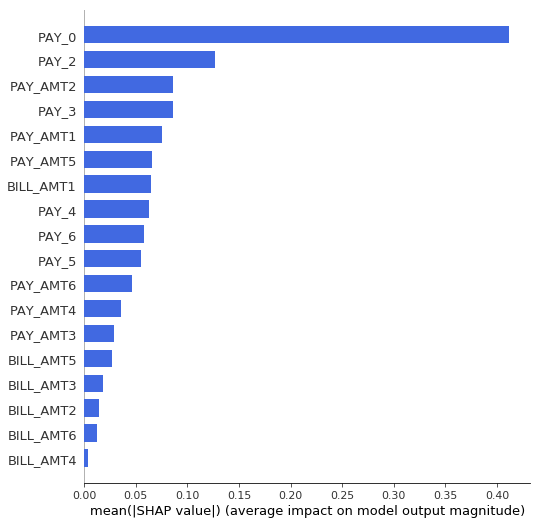
\includegraphics[height=0.8\linewidth, width=0.75\linewidth]{img/global_shap.png}
  		\caption{Global Shapley feature importance for $g_{\text{GBM}}$.}
  		\label{fig:global_shap}
	\end{subfigure}
	\begin{subfigure}{.5\textwidth} \centering
		\vspace{5pt}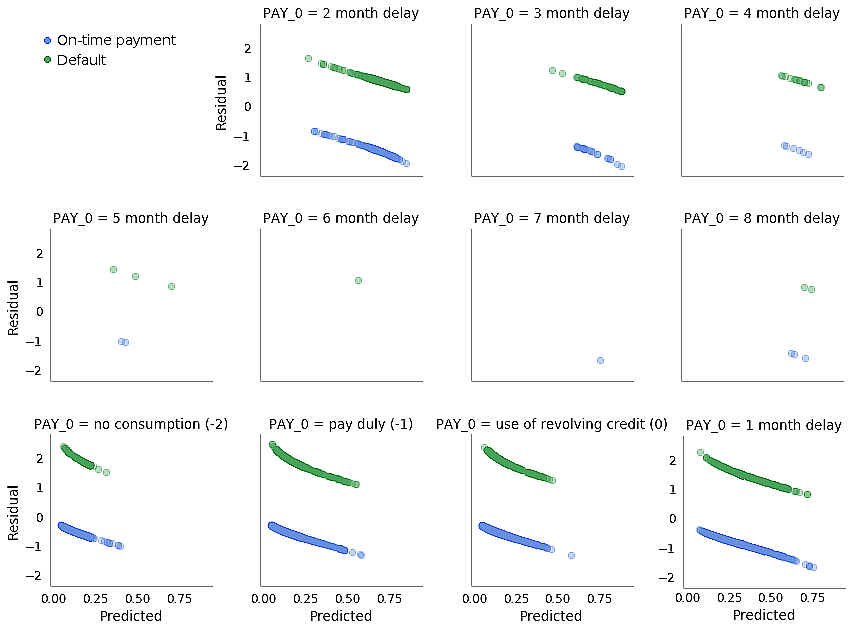
\includegraphics[width=0.85\linewidth]{img/resid.png}
  		\caption{$g_{\text{GBM}}$ deviance residuals and predictions by \texttt{PAY\_0}.}
  		\label{fig:resid}
	\end{subfigure}
	\vspace{-8pt}
	\caption{An unconstrained GBM probability of default model trained on the UCI credit card data\cite{uci}, $g_{\text{GBM}}$, generally over-emphasizes the importance of the input feature \texttt{PAY\_0}, a customer's most recent repayment status. $g_{\text{GBM}}$ produces large positive residuals when \texttt{PAY\_0} indicates on-time payments (\texttt{PAY\_0} $\leq$ 1) and large negative residuals when \texttt{PAY\_0} indicates late payments (\texttt{PAY\_0} $>$ 1). Combining explanatory and debugging techniques shows that $g_{\text{GBM}}$ is explainable, but probably not trustworthy. Code to replicate Figure \ref{fig:global_shap_resid} is available here: \url{https://github.com/h2oai/xai_guidelines}.} 
	\label{fig:global_shap_resid}
\end{figure*}

If trust in models is your goal, explanations alone are insufficient. Explanation, as a general idea, is related more directly to understanding and transparency than to trust.\footnote{The Merriam-Webster definition of \textit{explain}, accessed May 8\textsuperscript{th} 2019, does not mention \textit{trust}: \url{https://www.merriam-webster.com/dictionary/explain}.} Explanations enhance understanding directly (and trust as a side-effect when explanations are acceptable to human users). In short, ML can be understood and not trusted, and trusted but not understood:
\begin{itemize}
\item \textbf{Explanation \& understanding without trust}: In Figure \ref{fig:global_shap_resid}, global Shapley explanations and residual analysis identify a pathology in an unconstrained GBM model, $g_{\text{GBM}}$. In this example scenario, $g_{\text{GBM}}$ is explainable, but not trustworthy. 
\item \textbf{Trust without explanation \& understanding}: Years before reliable explanation methods were widely acknowledged and available, black-box models, such as autoencoder and MLP neural networks, were used for fraud detection in the financial services industry \cite{gopinathan1998fraud}. When these models performed well, they were trusted.\footnote{See: \url{https://www.sas.com/en_ph/customers/hsbc.html}, \url{https://www.kdnuggets.com/2011/03/sas-patent-fraud-detection.html}.} However, they were not explainable or well-understood by contemporary standards.  
\end{itemize}

\subsection{Guideline: Learn How Explainable ML is Used for Nefarious Purposes.} \label{sec:nefarious}

When used disingenuously, explainable ML methods can enable:
\begin{itemize}
\item Misuse or intentionally abuse of black-box ML \cite{fair_washing}, \cite{please_stop}.
\item Hacking or stealing of data and models through public prediction APIs or other endpoints \cite{membership_inference}, \cite{model_stealing}. 
\end{itemize}
\noindent Explainable ML methods may be used for additional unknown destructive purposes today, and are also likely to be used for other nefarious purposes in the future. 

\subsubsection{Corollary: Explainable ML Can be Used to Crack Nefarious Black-boxes.} Used as white-hat hacking tools, explainable ML can draw attention to fairness or accuracy problems in proprietary black-boxes. See \citet{angwin16} for evidence that cracking of commercial black-box models for oversight purposes is possible.\footnote{This text makes no claim on the quality of the analysis in Angwin et al. (2016), which has been criticized \cite{flores2016false}. This now infamous analysis is presented only as evidence that motivated activists can crack commercial black-boxes using surrogate models and other explanatory techniques. Moreover, such analyses would likely on improve with established best-practices for explainable ML.} 

\subsubsection{Corollary: Explainable ML is a Privacy Vulnerability.} Recent research shows that providing explanations along with predictions eases attacks that can compromise sensitive training data \cite{shokri2019privacy}. 

\subsection{Augment Surrogate Models with Direct Explanations.} \label{sec:surrogate}

\begin{figure*}[htb!]
	\begin{subfigure}{.55\textwidth}	\centering
		\includegraphics[height=0.5\linewidth, width=0.8\linewidth]{img/dt_surrogate.png}
  		\caption{Na\"ive $h_{\text{tree}}$, \textit{a surrogate model}, forms an approximate overall flowchart\\ for the explained model, $g_{\text{GBM}}$.}
  		\label{fig:dt_surrogate}
	\end{subfigure}\hfill
	\begin{subfigure}{.45\textwidth}	\centering
  		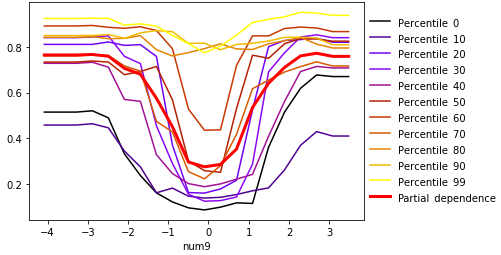
\includegraphics[height=0.4\linewidth, width=0.75\linewidth]{img/pdp_ice.png}
  		\caption{Partial dependence and ICE curves generated \textit{directly from the explained model}, $g_{\text{GBM}}$.}
  		\label{fig:pdp_ice}
	\end{subfigure} \vspace{-5pt}
	\caption{$h_{\text{tree}}$ displays known interactions in $f = X_{\text{num}1} * X_{\text{num}4} + |X_{\text{num}8}| * X_{\text{num}9}^2$ for $\sim -0.923 < X_{\text{num9}} <  \sim 1.04$. Modeling of the known interaction between $X_{\text{num9}}$ and $X_{\text{num8}}$ in $f$ by $g_{\text{GBM}}$ is confirmed by the divergence of partial dependence and ICE curves for $\sim -1 < X_{\text{num9}} <  \sim 1$. Explanations from a surrogate model have augmented and confirmed findings from a direct model visualization technique. Code to replicate Figure \ref{fig:pdp_ice_dt_surrogate} is available here: \url{https://github.com/h2oai/xai_guidelines}.}
	\label{fig:pdp_ice_dt_surrogate}
\end{figure*}

Models of models, or surrogate models, can be helpful explanatory tools, but they are often approximate, low-fidelity explainers. Combine direct explanation methods with approximate global or local summaries provided by surrogate models to enhance both types of explanations. In Figure \ref{fig:pdp_ice_dt_surrogate}, a surrogate decision tree and direct explanations, in the form of partial dependence and ICE, highlight and confirm modeled interactions \cite{art_and_sci}.

\subsubsection{Corollary: Augment LIME with Direct Explanations.} LIME can be combined with direct explanations to yield deeper insights.  Table \ref{tab:lime} contains LIME $h_{\text{GLM}}$ coefficients that can used along with the local Shapley feature contributions in Figure \ref{fig:dt_shap} to reason about the modeled average behavior for risky customers and to differentiate the behavior of any one specific risky customer from their peers under the model for debugging and compliance purposes.

\begin{table}[htb!]
	\caption{Coefficients for a local linear interpretable model, $h_{\text{GLM}}$, with an intercept of 0.77 and an $R^2$ of 0.73. $h_{\text{GLM}}$ is trained on a segment of the UCI credit card dataset containing higher-risk customers with late most recent repayment statuses, $\mathbf{X}_{PAY \_ 0 > 1}$, and the predictions of a simple decision tree, $g_{\text{tree}}(\mathbf{X}_{\text{PAY\_0} > 1})$. Code to replicate Table \ref{tab:lime} is available here: \url{https://github.com/h2oai/xai_guidelines}.} 
		\centering
			\footnotesize
				\begin{tabular}{ | p{2cm} | p{1.7cm} | }
				\hline
				$h_{\text{GLM}}$\newline Feature & $h_{\text{GLM}}$\newline Coefficient \\ 
				\hline
				\texttt{PAY\_0 == 4} & $0.0009$ \\
				\hline
				\texttt{PAY\_2 == 3} & $0.0065$ \\
				\hline
				\texttt{PAY\_5 == 2} & $-0.0006$ \\
				\hline
				\texttt{PAY\_6 == 2} & $0.0036$ \\
				\hline				
				\texttt{BILL\_AMT1} & $3.4339\mathrm{e}{-08}$ \\
				\hline
				\texttt{PAY\_AMT1} & $4.8062\mathrm{e}{-07}$ \\
				\hline	
				\texttt{PAY\_AMT3} & $-5.867\mathrm{e}{-07}$ \\	
				\hline	
			\end{tabular}	
  		\label{tab:lime}
\end{table}	

\subsection{Use Fully Transparent ML Mechanisms for High-Stakes Applications.} \label{sec:white_box}

Many high-stakes applications are regulated. Explanation, with interpretable models, model debugging, disparate impact analysis, and the documentation they enable, are often required under numerous regulatory statutes in the U.S. and E.U., and explainable ML tools are already used to document, explain, understand, and validate different types of models in the financial services industry \cite{lime-sup}, \cite{wf_xnn}.\textsuperscript{\ref{fn:regs}, \ref{fn:Chen},}\footnote{\scriptsize{This is \textit{already} happening: \url{https://www.prnewswire.com/news-releases/new-patent-pending-technology-from-equifax-enables-configurable-ai-models-300701153.html}.}}\\

\vspace{-8pt}
\noindent Aside from regulatory concerns, explanation enables logical appeal processes for incorrect decisions made by ML models. Consider being negatively impacted by an erroneous black-box model decision, say for instance being mistakenly denied a loan or parole. How would you argue your case for appeal without knowing how model decisions were made? \footnote{This too is happening \textit{today}. According to the New York Times, a man named Glenn Rodr\'iguez found himself in this unfortunate position in a penitentiary in Upstate New York in 2016: \url{https://www.nytimes.com/2017/06/13/opinion/how-computers-are-harming-criminal-justice.html}.}

\begin{figure*}[htb!]
	\begin{subfigure}{.55\textwidth}
		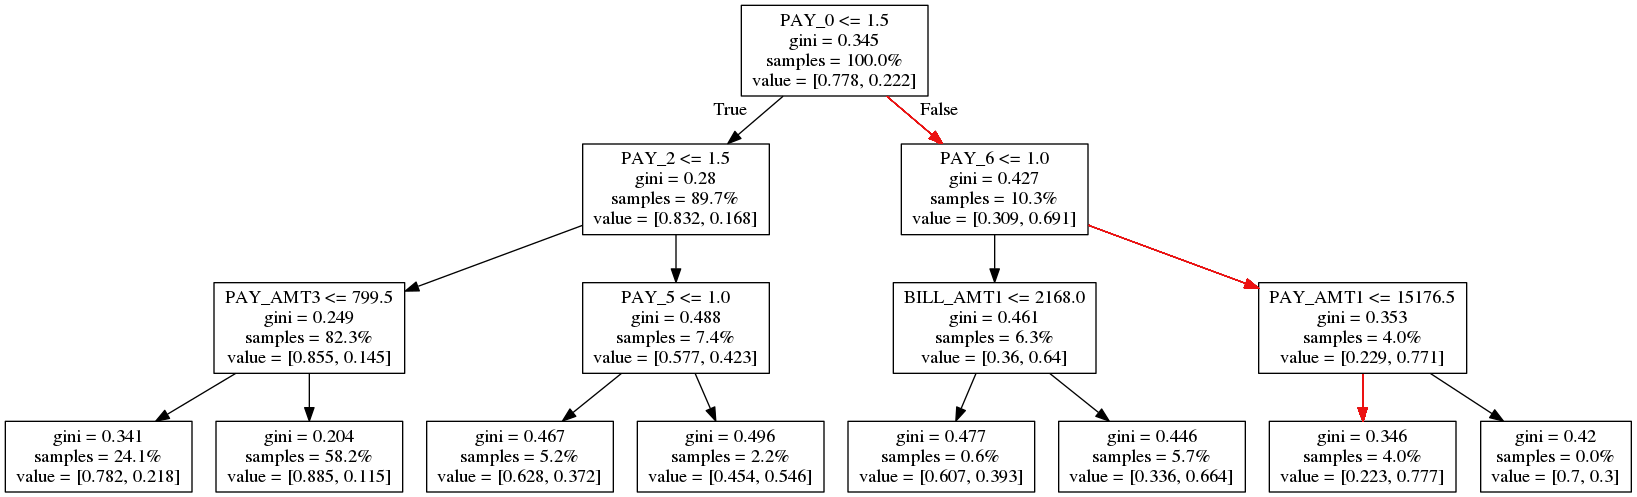
\includegraphics[height=.45\linewidth, width=1.15\linewidth]{img/dt.png}
  		\caption{Simple decision tree, $g_{\text{tree}}$, trained on the UCI credit card data to predict default with validation AUC of 0.74. The decision policy for a high-risk individual is highlighted in red.}
  		\label{fig:dt}
	\end{subfigure}\hspace*{40pt}
	\vspace{25pt}\begin{subfigure}{.45\textwidth}
  		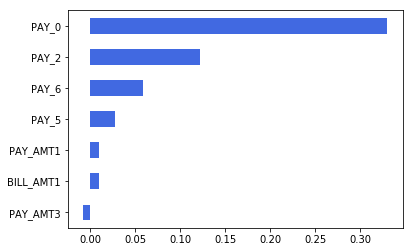
\includegraphics[height=.5\linewidth, width=.8\linewidth]{img/shap.png}
		\caption{Locally-accurate Shapley contributions for the\\ highlighted individual's probability of default.}
  		\label{fig:shap}
	\end{subfigure}\vspace{-30pt}
	\caption{A simple decision tree, $g_{\text{tree}}$, is trained on the UCI credit card dataset to predict probability of default. $g_{\text{tree}}$ has a validation AUC of 0.74. The decision-policy for a high-risk customer is highlighted in \ref{fig:dt} and the locally-accurate Shapley contributions for this same individual's predicted probability are displayed in \ref{fig:shap}. The Shapley values are helpful because they highlight the local importance of features not on the decision path in this particular encoding of the unknown signal-generating function, i.e. $g_{\text{tree}}$, which could be underestimated by examining the decision policy alone. Code to replicate Figure \ref{fig:dt_shap} is available here: \url{https://github.com/h2oai/xai_guidelines}.} 
	\label{fig:dt_shap}
\end{figure*}

\subsubsection{Corollary: Use Interpretable Models Along with Explanation Techniques.} Interpretable models and explanations can be used together in a holistic ML workflow as illustrated in Figure \ref{fig:hc_ml}. Figure \ref{fig:dt_shap} displays a globally interpretable model and accurate numeric feature contributions for a model prediction. Even for interpretable models, such as linear models and decision trees, Shapley values present accuracy and consistency advantages over standard feature attribution methods \cite{lipovetsky2001analysis}, \cite{tree_shap}, \cite{shapley}. 

\subsubsection{Corollary: Use Explanations Along with Bias Testing and Remediation.} In banks, using post-hoc explanatory tools along with disparate impact analysis is necessary to comply with model documentation guidance and with fair lending regulations.\textsuperscript{\ref{fn:Chen},}\footnote{\scriptsize{See: \url{https://www.aba.com/Compliance/Documents/FairLendingWhitePaper2017Apr.pdf}.}}\textsuperscript{,}\footnote{\scriptsize{See: \url{https://www.govinfo.gov/content/pkg/FR-1994-04-15/html/94-9214.htm}.}} 

\subsubsection{Corollary: Explanation is Not a Frontline Fairness Tool.} In many high-stakes and commercially viable applications of explainable ML in credit lending, insurance, and employment in the U.S. that fall under FCRA, ECOA, or other applicable regulations, demographic attributes cannot be used in predictive models and thus their contribution to model predictions cannot be explained using common explainable ML techniques. Even when demographic attributes can be used in predictive models, it has been shown that explanations may not detect unwanted social bias \cite{fair_washing}. Given these known drawbacks, it is recommended that fairness techniques are used to test for and remediate unwanted sociological bias, and explanations are used to augment and understand bias when appropriate.  

\subsubsection{Corollary: Use Bias Testing  Along with Constrained Models.} Because unconstrained ML models have the ability to treat similar individuals differently based on small differences in their data values, unconstrained models can cause local bias that is not detectable with standard bias testing methods that analyze group fairness \cite{dwork2012fairness}. To minimize local unwanted sociological bias when using machine learning, and to ensure standard bias testing methods are most effective, pair bias testing techniques with constrained models.

\section{Conclusion: A Holistic ML Approach} \label{sec:conclusion}

ML is used today to make life-altering decisions about employment, bail, parole, and lending.\footnote{ICLR 2019 model debugging workshop CFP: \url{https://debug-ml-iclr2019.github.io/}.} The scope of decisions delegated to ML systems seems likely only to expand in the future. By presenting explainable ML guidelines, this tutorial also gives examples of combining innovations from several sub-disciplines of ML research to train explainable, fair, and trustable predictive modeling systems. As proposed in Figure \ref{fig:hc_ml}, using these techniques together can create a more holistic approach to ML, potentially better-suited for use in business- and life-critical decision support than conventional workflows.

\begin{figure}[htb!]
	\begin{center}
		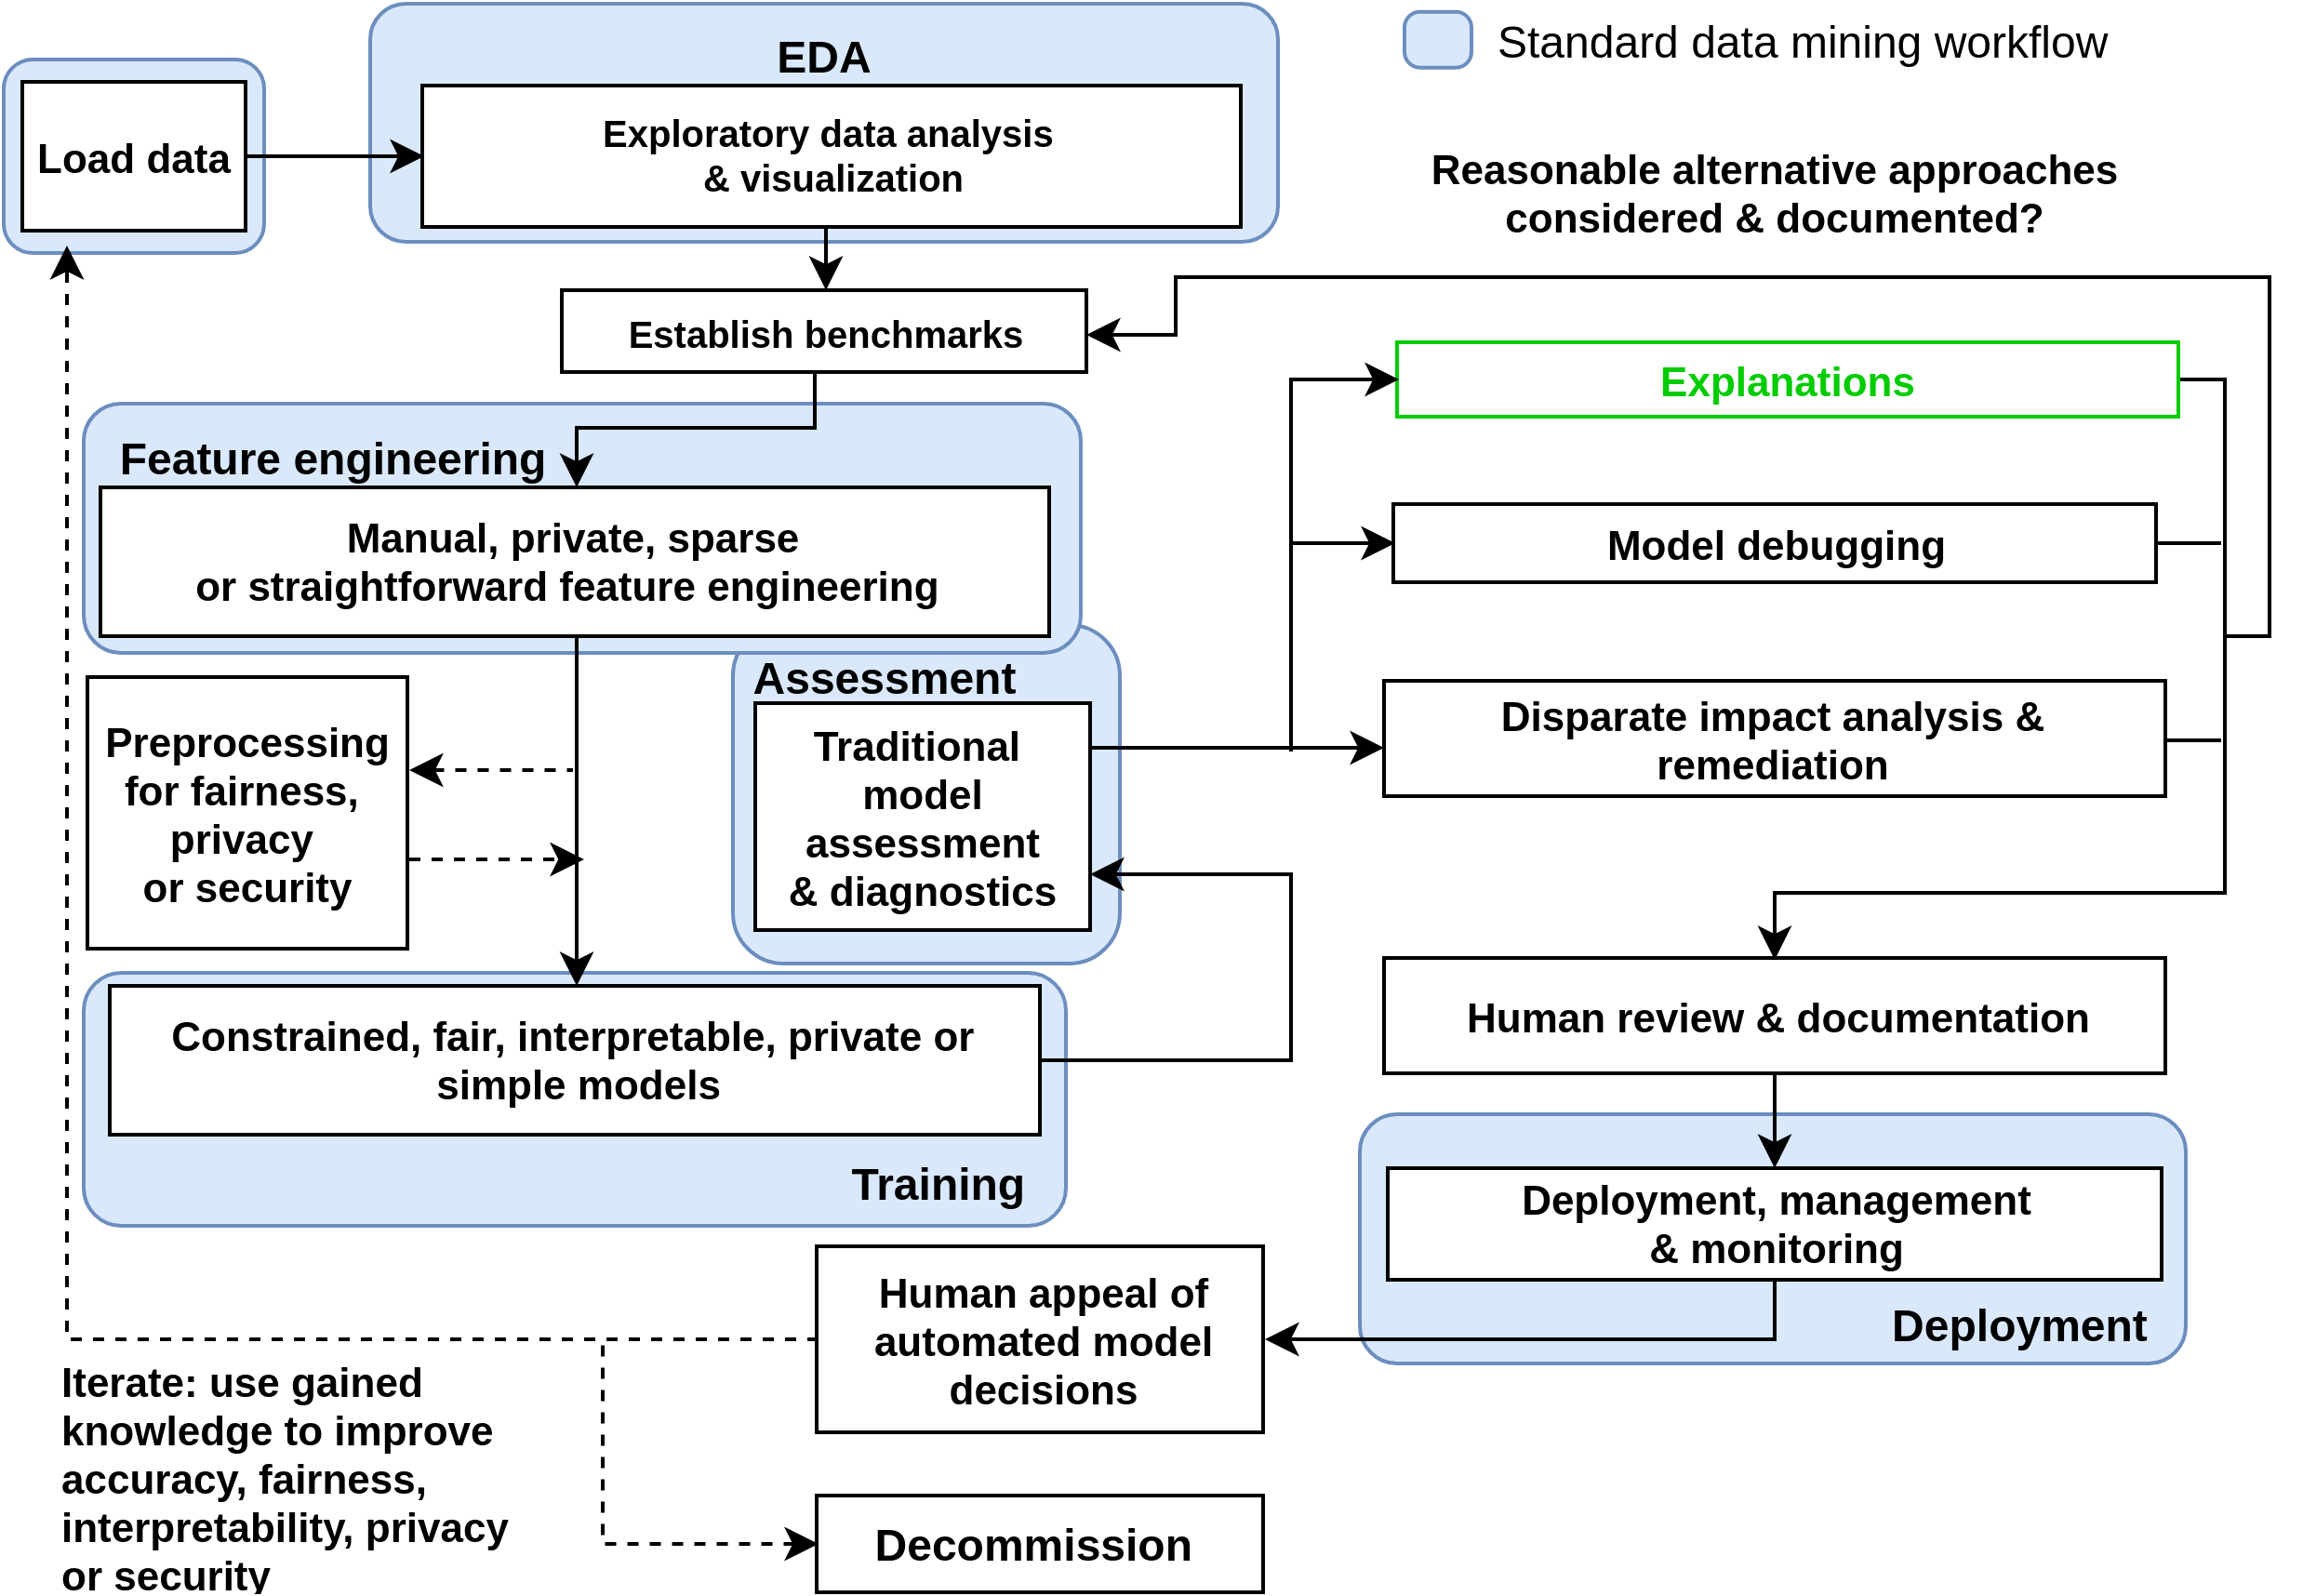
\includegraphics[scale=0.1]{img/hc_ml.png}
		\caption{A diagram of a proposed holistic ML workflow in which explanations (highlighted in green) are used along with interpretable models, bias testing and remediation techniques, and other review and appeal mechanisms to create a fair, accountable, and transparent ML system.}
		\label{fig:hc_ml}
	\end{center}
\end{figure}

\section*{Software Resources}

This tutorial uses Jupyter notebooks and Python code stored in a public GitHub repository with an Apache 2.0 license \url{https://github.com/h2oai/xai_guidelines}. Notebooks will be deployed in H2O.ai's free educational cloud environment, Aquarium: \url{http://aquarium.h2o.ai}. Attendees will only need an email address (to receive a password after Aquarium registration) and to bring their laptop to access and execute the materials. 


% The next two lines define the bibliography style to be used, and the bibliography file.
\bibliographystyle{ACM-Reference-Format}
\clearpage
\footnotesize
\bibliography{responsible_xai}

\end{document}
